\documentclass{assignment}
\title{5370 Midterm}

\begin{document}

\textbf{3.}
\label{SquishyBear}
The average word in English is $\lambda =5.1$ letters.
\begin{enumerate}
\item  If letters are drawn randomly from an $N=27$ character alphabet (A through Z and a space),\footnote{
    We are not considering punctuation, capitalization or numbers.
  }
  then when is a thick novel with $W$ words typical? Explain your reasoning. \\

  \textbf{Solution:} \\
  When
  \begin{align}
    p\left(X^{\ceil{W*(5.1 + 1)}}\right) & \approx 2^{-W*(5.1 + 1)*(5.1 + 1)} \label{problem3_1}
  \end{align}
  Because when n is very large, $E\left[\df{1}{n}l(X^n)\right] \approx H(X)$, which means $H(X) \approx \lambda$. The number of alphabets
  here, including space, should be about $\ceil{W * (\lambda + 1)}$, where ``+1'' is due the space character. Since
  we are adding space at the end of each words, the entropy for words with space should be $\lambda + 1$. So we have
  (\ref{problem3_1}), satisfying which makes the sequence at least weakly typical.

\item Here is a web page of 40,000 sampled words
  \begin{center}
    \verb"http://www.math.cornell.edu/~mec/2003-2004/cryptography/subs/frequencies.html"
  \end{center}
  \begin{enumerate}
  \item Complete the {\bf Count} column in table by including the {\em space}. Call the resulting empirical
    distribution $q(x)$ where $x=0,1,2,\cdots$ corresponds to (space, e, t, a, o, $\cdots$). \\
    \textbf{Solution:} \\
    Since sampled words are 40000, there should be the same amount of spaces, one space per word.

    \begin{tabular}[h]{l|l|r|r}
      Index & Letters & Count & Probability\\
      \hline
      0     & Space   & 40000 & 0.1799\\
      1     & E       & 21912 & 0.09857\\
      2     & T       & 16587 & 0.07461\\
      3     & A       & 14810 & 0.06662\\
      4     & O       & 14003 & 0.06300\\
      5     & I       & 13318 & 0.05991\\
      6     & N       & 12666 & 0.05698\\
      7     & S       & 11450 & 0.05151\\
      8     & R       & 10977 & 0.04938\\
      9     & H       & 10795 & 0.04856\\
      10    & D       & 7874  & 0.03542\\
      11    & L       & 7253  & 0.03263\\
      12    & U       & 5246  & 0.02360\\
      13    & C       & 4943  & 0.02224\\
      14    & M       & 4761  & 0.02142\\
      15    & F       & 4200  & 0.01889\\
      16    & Y       & 3853  & 0.01733\\
      17    & W       & 3819  & 0.01718\\
      18    & G       & 3693  & 0.01661\\
      19    & P       & 3316  & 0.01492\\
      20    & B       & 2715  & 0.01221\\
      21    & V       & 2019  & 0.009082\\
      22    & K       & 1257  & 0.005654\\
      23    & X       & 315   & 0.001417\\
      24    & Q       & 205   & 0.0009222\\
      25    & J       & 188   & 0.0008457\\
      26    & Z       & 128   & 0.0005758
    \end{tabular} \\

    After experiment, I found that beta-binomial distribution with $n=26, \alpha=0.68, \beta=2.7$ fit the data the best
    as shown in fig~\ref{fig:beta-binomial-fit}. Exponential distribution also fits well, but not as well as
    beta-binomial distribution, also exponential distribution is continuous, and beta-binomial is discrete which also
    make beta-binomial distribution a better fit.
    \begin{figure}[!h]
      \centering
      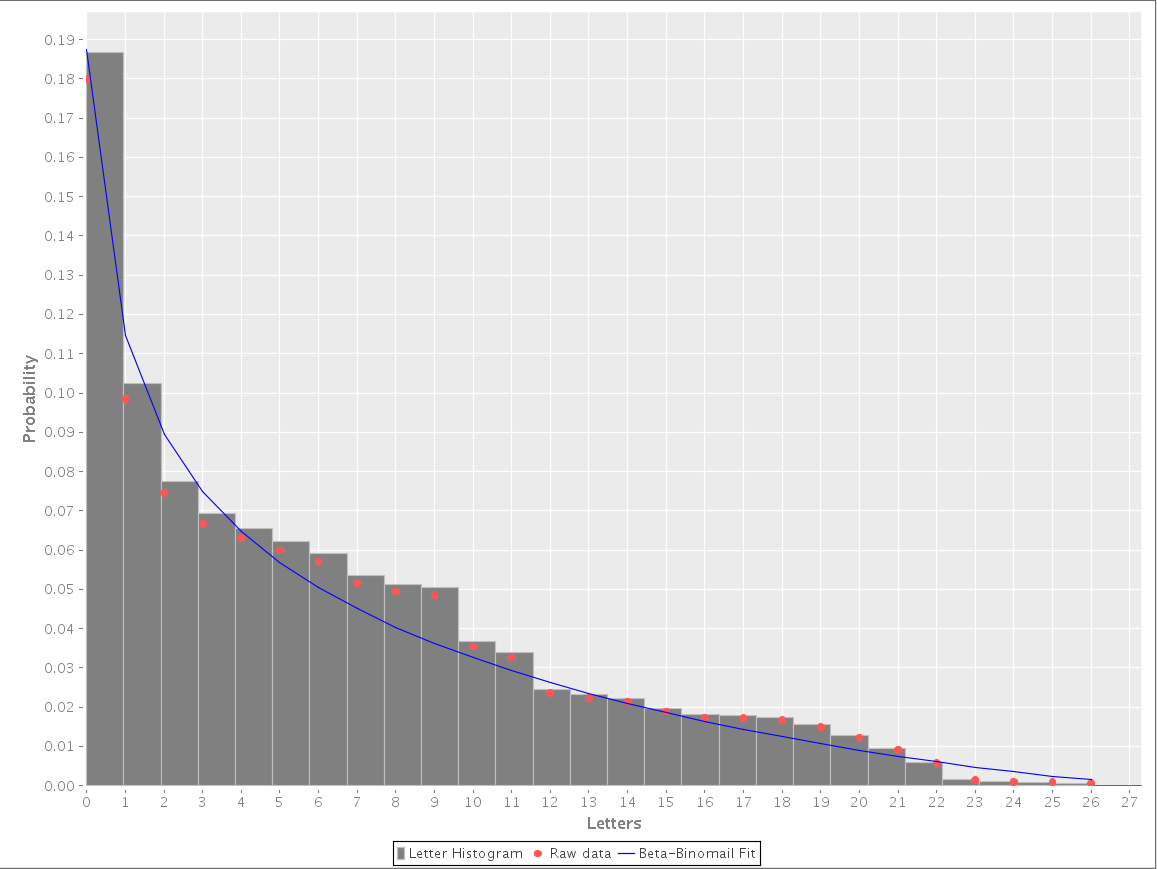
\includegraphics[width=5in]{pics/beta_binomial_fit.eps}
      \caption{Beta-binomial pmf fitting with $n=26, \alpha=0.68, \beta=2.7$}
      \label{fig:beta-binomial-fit}
    \end{figure}

  \item Find the value of $\alpha$ that minimizes the Kullback-Liebler distance between the distribution corresponding
    to this augmented table and
    \begin{align}
      p(x) = (1-\alpha) \alpha^x \label{eq:p3b_p(x)}
    \end{align}
    $$ $$ \\
    \textbf{Solutions:}\\
    Beta-binomial distribution pmf:
    \begin{align*}
      q(x|n, \alpha, \beta) & = \dbinom{n}{x} \df{B(x+\alpha, n-x+\beta)}{B(\alpha, \beta)} \\
      p(x) & = (1 - \alpha)\alpha^x
    \end{align*}
    Since we are assuming $q(x)$ as our true distribution and trying to make $p(x)$ as close to $q(x)$ as possible,
    by reducing KLIC, thus Kullback-Liebler distance should be expressed as:
    \begin{align*}
      D(q||p) & = \sum_x q(x)\log \df{q(x)}{p(x)} \\
      \shortintertext{Let}
      C_x & = \dbinom{n}{x} \\
      B_x & = B(x+\alpha, n-x+\beta) \\
      B   & = B(\alpha, \beta) \\
      \shortintertext{then we have:}
      D(q||p) & = \sum_x \dbinom{n}{x} \df{B(x+\alpha, n-x+\beta)}{B(\alpha, \beta)}
                \log \left(\df{\dbinom{n}{x} \df{B(x+\alpha, n-x+\beta)}{B(\alpha, \beta)}}{(1-\alpha)\alpha^x}\right) \\
              & = \df{1}{B}\sum_x C_xB_x\log\left( \df{\df{C_x B_x}{B}}{(1-\alpha)\alpha^x} \right) \\
              & = \df{1}{B}\sum_x \left[C_xB_x\log\left(\df{C_xB_x}{B}\right) - C_xB_x\log ((1-\alpha)\alpha^x)\right] \\
              & = \df{1}{B}\sum_x C_xB_x\log\left(\df{C_xB_x}{B}\right) - \df{1}{B}\sum_x C_xB_x\log ((1-\alpha)\alpha^x)
    \end{align*}
    As we can see, the function of $D(q||p)$ contains a inverted log function with respect to $\alpha$. Since log is a
    concave function, if there is a critical point exist, it must be a global minima. To find the critical point, we
    need to set $\df{d}{d\alpha} D(q||p) = 0$
    \begin{align*}
      \df{d}{d\alpha} D(q||p)
      & = \df{d}{d\alpha} \left(\df{1}{B}\sum_x C_xB_x\log\left(\df{C_xB_x}{B}\right)
                                - \df{1}{B}\sum_x C_xB_x\log ((1-\alpha)\alpha^x)\right) = 0 \\
      & = - \df{1}{B}\sum_x\df{C_xB_x(x\alpha^{(x-1)}-(x+1)\alpha^{x})}{(1-\alpha)\alpha^x} = 0\\
      & = - \df{1}{B}\sum_x\df{C_xB_x(x\alpha^{-1}-x-1)}{(1-\alpha)} = 0 \\
      & = \sum_x C_xB_x(x\alpha^{-1}-x-1) = 0 \\
      & = \sum_x C_xB_xx - \sum_x C_xB_x \alpha x - \sum_x C_xB_x\alpha = 0 \\
      \alpha & = \df{\sum_{x=0}^{26} C_xB_xx}{\sum_{x=0}^{26} C_xB_x (x + 1)}
               = \df{\sum_{x=0}^{26} \dbinom{n}{x}B(x+\alpha, n-x+\beta) x}
                    {\sum_{x=0}^{26} \dbinom{n}{x}B(x+\alpha, n-x+\beta) (x + 1)} \\
      \shortintertext{with $n=26, \alpha=0.68, \beta=2.7$}
      \alpha & \approx 0.8395
    \end{align*}

    % \begin{align*}
    %   q(x) & = \df{\lambda^x}{x!}e^{-\lambda} = \df{\lambda^x}{x! e^{\lambda}} \\
    %   p(x) & = (1-\alpha) \alpha^x
    % \end{align*}
    % \begin{align*}
    %   D(p||q) & = \sum_x p(x)\log \df{p(x)}{q(x)}\\
    %           & = \sum_{x=0}^{26} (1-\alpha) \alpha^x \log \df{x!e^{\lambda}(1-\alpha) \alpha^x}{\lambda^x} \\
    %           & = \sum_{x=0}^{26} \left[(1-\alpha) \alpha^x\log \df{x!e^{\lambda}}{\lambda^x}
    %             + (1-\alpha) \alpha^x\log (1-\alpha) \alpha^x\right]
    % \end{align*}
    % Since this is a function contains an odd degree of polynomial function, $\left.a^{x+1}\right|_{x=26}$, this function
    % has no global minimum or global maximum. So we have to use (\ref{eq:p3b_p(x)}) as our true distribution.

    % \begin{align*}
    %   D(p||q) & = \sum_x p(x)\log \df{p(x)}{q(x)}\\
    %        & = \sum_{x=0}^{26} (1-\alpha) \alpha^x \log \df{x!e^{\lambda}(1-\alpha) \alpha^x}{\lambda} \\
    %   \shortintertext{for $x=0$:}
    %   \df{d}{d\alpha}\left((1-\alpha) \log\df{e^{\lambda}(1 - \alpha)}{\lambda}\right)
    %           & = -\log\df{e^{\lambda}(1 - \alpha)}{\lambda}
    %             - \df{e^{\lambda}(1 - \alpha)}{\lambda} \df{\lambda}{e^{\lambda}(1 - \alpha)} \\
    %           & = -\log\df{e^{\lambda}(1 - \alpha)}{\lambda} - 1 \\
    %  \end{align*}
    %  \begin{align*}
    %   \shortintertext{for $x = 1, 2, \dots, 26$, let:}
    %   T & = (1-\alpha) \alpha^x \log \df{x!e^{\lambda}(1-\alpha) \alpha^x}{\lambda} \\
    %        & = \alpha^x\log \df{x!e^{\lambda}(1-\alpha) \alpha^x}{\lambda} -
    %          \alpha^{x+1}\log \df{x!e^{\lambda}(1-\alpha) \alpha^x}{\lambda} \\
    %   \df{d}{d\alpha} T
    %        & = xa^{x-1}\log \df{x!e^{\lambda}(1-\alpha) \alpha^x}{\lambda}
    %          + a^x \left( \df{x!e^{\lambda}}{\lambda} \right)
    %          \df{(-a^x + x(1 - \alpha)\alpha^{x-1})\lambda}{x!e^{\lambda}(1-\alpha) \alpha^x} \\
    %        & \quad - (x+1)\alpha^x\log \df{x!e^{\lambda}(1-\alpha) \alpha^x}{\lambda}
    %          - a^{x+1} \left( \df{x!e^{\lambda}}{\lambda} \right)
    %          \df{(-a^x + x(1 - \alpha)\alpha^{x-1})\lambda}{x!e^{\lambda}(1-\alpha) \alpha^x} \\
    %        & = xa^{x-1}\log \df{x!e^{\lambda}(1-\alpha) \alpha^x}{\lambda}
    %          + \df{-a^x + x \alpha^{x-1} - x\alpha^x}{(1-\alpha)} \\
    %        & \quad - (x+1)\alpha^x\log \df{x!e^{\lambda}(1-\alpha) \alpha^x}{\lambda}
    %          - \df{-a^{x+1} + x(1 - \alpha)\alpha^{x}}{1-\alpha} \\
    %        & = (x a^{x-1} - (x+1) \alpha^x)\log \df{x!e^{\lambda}(1-\alpha) \alpha^x}{\lambda}
    %          + \df{-a^x + x \alpha^{x-1} - x\alpha^x + a^{x+1} - x(1 - \alpha)\alpha^{x}}{1-\alpha}
    % \end{align*}

    % \begin{align*}
    %   D(q || p) & = \sum_x q(x) \log \df{q(x)}{p(x)} \numberthis \label{eq:p3b_KLD}\\
    %             & = \sum_x \df{\lambda}{x!e^{\lambda}}\log \df{\lambda}{x!e^{\lambda} (1-\alpha)\alpha^x} \\
    %             & = \sum_x \df{\lambda}{x!e^{\lambda}}(\log \lambda - \log (x! e^{\lambda}(1 - \alpha) \alpha^x)) \\
    %             & = \df{27\lambda}{x!e^{\lambda}} - \sum_{x=0}^{26} \log (x! e^{\lambda}(1 - \alpha) \alpha^x)
    % \end{align*}
    % Since log is a concave function and this particular one is a inverted log function, if there is a point where
    % derivative is 0, it must be a global minimum.
    % \begin{align*}
    %   \df{d}{d\alpha} D(q || p) & = - \sum_{x=0}^{26} \df{x x!e^{\lambda}a^{x-1} - (x+1)!e^{\lambda}a^x}
    %                                                     {x!e^{\lambda}(1-\alpha)\alpha^x} \\
    %                             & = - \sum_{x=0}^{26} \df{x a^{-1} - (x+1)}{1-\alpha} \\
    %                             & = \df{\sum_{x=0}^{26}[x - \alpha(x + 1)]}{\alpha^2 - \alpha} = 0 \\
    %   \sum_{x=0}^{26}[x - \alpha(x + 1)] & = 0 \\
    %   \alpha\sum_{x=0}^{26}(x + 1) & = \sum_{x=0}^{26} x \\
    %   \alpha & = \df{\sum_{x=0}^{26} x}{\sum_{x=0}^{26}(x + 1)} = \df{13}{14}
    % \end{align*}
    % So, when $\alpha = \frac{13}{14}$, (\ref{eq:p3b_KLD}) has the smallest value.

  \item Compare this to the $\alpha$ that minimizes
    $$ \sum_{x=0}^\infty \left| p(x) -  q(x) \right|^2 $$ \\
    \textbf{Solution:} \\
    Since we only have $0-26$, i.e., 26 alphabets with one space character, the summation would only go up to 26, reset
    of terms would be all 0
    \begin{align*}
      \sum_{x=0}^{26} \left| p(x) -  q(x) \right|^2
      & = \sum_{x=0}^{26} \left| (1- \alpha) \alpha^x - \df{C_xB_x}{B}\right|^2 \\
      & = \sum_{x=0}^{26} \left| a^x - a^{x+1} - \df{C_xB_x}{B}\right|^2 \\
      & = \sum_{x=0}^{26} \left(  a^{2x} - a^{2x+1} - \df{C_xB_x}{B}a^x \right. \\
      & \quad \quad \quad \quad - a^{2x+1} + a^{2x+2} + \df{C_xB_x}{B}a^{x+1} \\
      & \quad \quad \quad \quad \left. - \df{C_xB_x}{B}a^{x} + \df{C_xB_x}{B}a^{x+1} + \left(\df{C_xB_x}{B}\right)^2
        \right) \\
      & = \sum_{x=0}^{26} \left(a^{2x+2} - 2a^{2x+1} + a^{2x} + \df{2C_xB_x}{B}a^{x+1} - \df{2C_xB_x}{B}a^{x} +
        \left(\df{C_xB_x}{B} \right)^2 \right) \numberthis \label{eq:prob3c:f}\\
      & = \sum_{x=0}^{26} \left(a^{2x+2} - 2a^{2x+1} + a^{2x}\right)
        + \sum_{x=0}^{26} \left( \df{2C_xB_x}{B}a^{x+1} - \df{2C_xB_x}{B}a^{x} +
        \left(\df{C_xB_x}{B} \right)^2 \right) \numberthis \label{eq:prob3c:f3}\\
      % & = \sum_{x=0}^{26} \left((a - 1)^2 a^{2x}  + \df{2C_xB_x}{B} a^{x+1} - \df{2C_xB_x}{B} a^x
      %   + \left(\df{C_xB_x}{B}\right)^2\right) \\
      % & = \sum_{x=0}^{26} a^{2x}(a - 1)^2
      %   + \sum_{x=0}^{26} \left(  \df{2C_xB_x}{B} a^{x+1} - \df{2C_xB_x}{B} a^x + \left(\df{C_xB_x}{B}\right)^2\right) \\
      % & = \sum_{x=0}^{26} (a^{2x+2} - 2a^{2x+1} + a^{2x})
      %   + \sum_{x=0}^{26} \left( 2C_xB_x a^{x+1} - 2C_xB_x a^x + \df{(C_xB_x)^2}{B}\right)
      %   \numberthis \label{eq:prob3c:f2} \\
    \end{align*}
    Since this is a polynomial with even degree and positive leading coefficient, $a^{2\times 26 + 2} = a^{54}$, the
    opening of the polynomial should be upward and it should have at least one global minimum.

    With first and second derivative of (\ref{eq:prob3c:f}):
    \begin{align*}
      \df{d}{da}\left(\sum_{x=0}^{26} \left| p(x) -  q(x) \right|^2\right)
      & = \sum_{x=1}^{26} \left( (2x+2)a^{2x+1} - (4x+2)a^{2x} + 2xa^{2x-1}\right) \\
      & \quad + \sum_{x=1}^{26} \left( (x+1)\df{2C_xB_x}{B} a^{x} - x\df{2C_xB_x}{B} a^{x-1}\right)
        + 2a -2 + \df{2C_0B_0}{B} \\
      \df{d^2}{da^2}\left(\sum_{x=0}^{26} \left| p(x) -  q(x) \right|^2\right)
      & = \sum_{x=2}^{26}  \left((2x+2)(2x+1)a^{2x} - (2x+2)2xa^{2x-1} + 2x(2x-1)a^{2x-2}\right) \\
      & \quad  + \sum_{x=2}^{26} \left( x(x+1)2\df{C_xB_x}{B} a^{x-1} - x(x-1)2\df{C_xB_x}{B} a^{x-2}\right) \\
      & \quad + 12a^2 - 12a + 2 + \df{4C_1B_1}{B} + 2
    \end{align*}
    we can numerically find the global minimum(s) with Newton's
    method\footnote{\url{https://en.wikipedia.org/wiki/Newton\%27s_method}} which gives me $\alpha \approx 0.83495$.
    Code used for newton's method is shown
    in listing (\ref{lst:newton}) and (\ref{lst:binomial})
    \SourceCode{clojure}{Functions for using newton's method}{lst:newton}{../../src/elc5370/optimization.clj}
    \SourceCode{clojure}{Functions for beta binomial distribution}{lst:binomial}{../../src/elc5370/binomial.clj}
    % \begin{align*}
    %   & = (a - 1)^2\sum_{x=0}^{26} 2xa^{2x-1} + \df{1}{B}\sum_{x=0}^{26} \left(2C_xB_x(x+1)a^{x} - 2C_xB_xxa^{x-1}\right)
    % \end{align*}

  \item What is the average word length in English based on $q(x)$? On $p(x)$? \\
    \textbf{Solution:} \\
     Ideally,
     \begin{align*}
       \text{average word length} & = \df{\text{total length (or non-space characters count)}}
                                         {\text{number of words (or spaces)}}
                                    = \df{\text{182303}}{\text{40000}}
                                    \approx 4.56
     \end{align*}
     However, average length based on a distribution $f(x)$, in general, should be
     \begin{align*}
       \text{average word length} & = \df{\sum_{x=1}^{26} f(x)}{f(x=0)}
     \end{align*}
     So, for $q(x)$, we have:
     \begin{align*}
       \text{average word length} & = \df{\sum_{x=1}^{26} q(x)}{q(0)} \approx \df{0.8066}{0.1935} \approx 4.17 \\
       \shortintertext{where}
       q(x) & = \dbinom{n}{x} \df{B(x+\alpha, n-x+\beta)}{B(\alpha, \beta)}
              \quad \text{with $n = 26, \alpha = 0.68, \beta = 2.7$}
     \end{align*}
     For $p(x)$, we have:
     \begin{align*}
       \text{average word length} & = \df{\sum_{x=1}^{26} p(x)}{p(0)} \approx \df{0.8306}{0.1605} \approx 5.18 \\
       \shortintertext{where}
       p(x) & = (1- \alpha)\alpha^x \quad \text{with $\alpha$ = 0.8395}
     \end{align*}
  \end{enumerate}
\end{enumerate}


\end{document}
